\chapter{Információs technológiai infrastruktúrák}
\section{A klasszikus IT infrastruktúra}
A klasszikusnak mondott IT infrastruktúrát az írás korábbi részében már bemutattam. Itt most a háromrétegű architektúra egyes rétegeinek skálázását, megbízhatósági szintjének növelésére adott lehetőségeket szeretném bemutatni.
\subsection{Adatbázis réteg}
\todo{Klaszterek, replikák, stb.}
\subsection{Alkalmazás réteg}
\todo{PHP, Java skálázás?}
\subsection{Webkiszolgáló réteg}
\todo{Loadbalancing} 
\section{Felhőalapú infrastruktúrák}
\subsection{Mi is az a ,,számítási felhő''?}

A ,,számítási felhő'' (angolul \foreignlanguage{english}{cloud computing}) egy modell kényelmes, hálózaton keresztül hozzáférhető, konfigurálható számítási erőforrások (pl. hálózat, szerverek, tárhelyek, alkalmazások és szolgáltatások) egy megosztott készletének elérhetőségére, mely erőforrásokat minimális intézkedési erőfeszítéssel vagy szolgáltatói közbenjárással gyorsan rendelkezésre lehet bocsátani \cite{nistsp800-145}.

\todo{Lehet, hogy még finomítani kell a fordításon!}

\begin{comment}
Cloud computing is a model for enabling ubiquitous, convenient, on-demand network access to a shared pool of configurable computing resources (e.g., networks, servers, storage, applications, and services) that can be rapidly provisioned and released with minimal management effort or service provider interaction. 
\end{comment}

Általában hivatkozás szintjén nincsenek elkülönítve az Interneten keresztül szolgáltatott alkalmazások, és a felhő infrastrukturális részét képező hardverek, szoftverek, amelyek ezeket az alkalmazásokat elérhetővé teszik. Ahogy azt \aref{fig:cloud_computing_hu}.~ábrán is szemléltetni próbálom a felhő részét képezi az alkalmazás, szolgáltatás, és a hardver is.

\begin{figure}[h!]
\centering
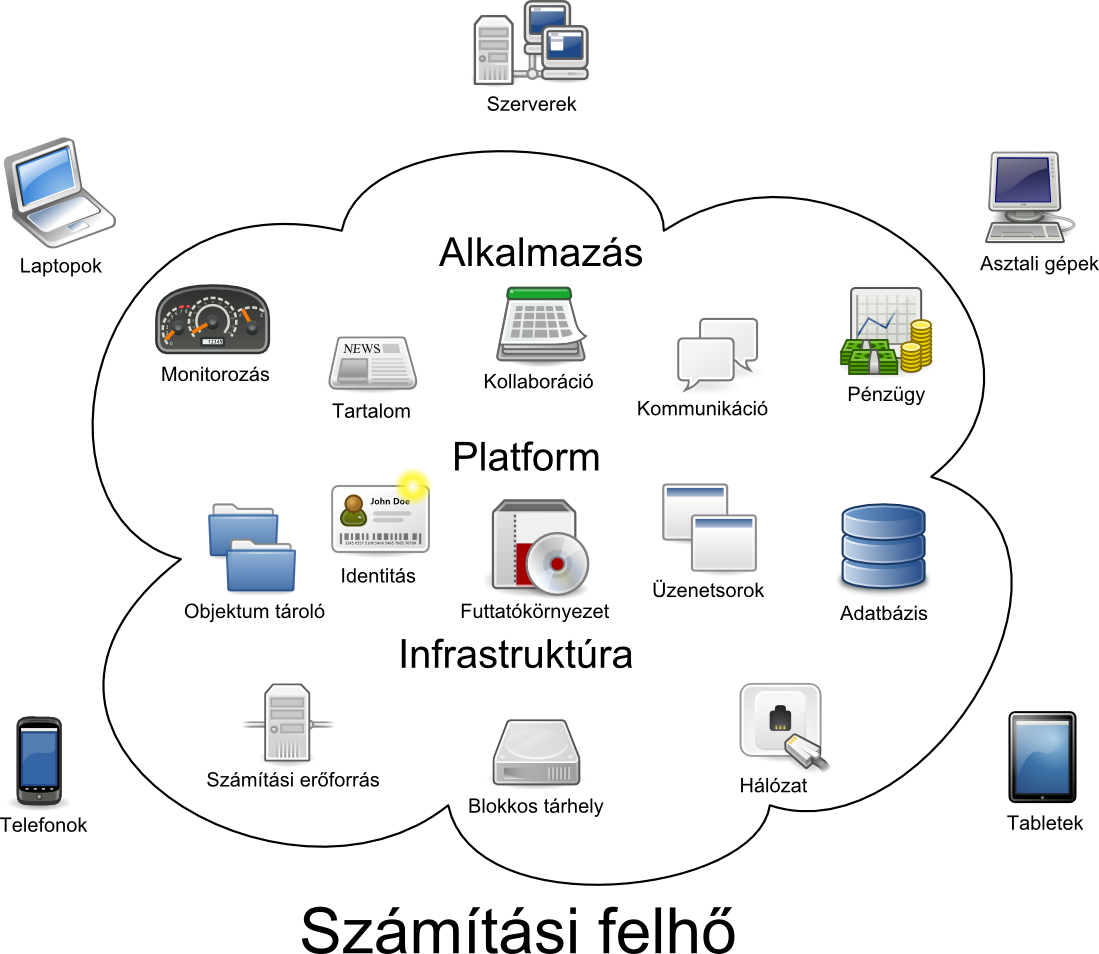
\includegraphics[width=0.80\textwidth]{figures/Cloud_computing_hu.png}
\caption{A számítási felhő (\foreignlanguage{english}{cloud computing}) (Forrás: \href{https://en.wikipedia.org/wiki/File:Cloud\_computing.svg}{Wikipedia})} \label{fig:cloud_computing_hu}
\end{figure}

Mélyebb elemzés során azonban a felhőt rétegekre lehet bontani, amely rétegeket a következő alfejezetben részletezném.

\subsection{A felhő szolgáltatási modelljei}

A felhő napjainkban négy szolgáltatási modellt tartalmaz, amelyek valamilyen szinten egymásra épülnek, ám nem feltétlenül határolhatóak el egzaktul egymástól. \Aref{fig:cloud_retegek}.~ábrán a felhő egy réteges felosztás látható, amely körülbelül azt hivatott kifejezni, hogy alulról fölfelé hogyan csökken a szolgáltatások felhasználó által igénybe vehető része.

\todo{Ez így lehet értelmetlen!} 

\begin{figure}[h!]
\centering
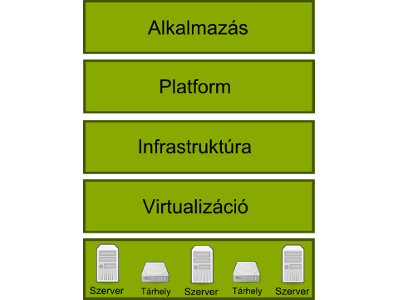
\includegraphics[width=0.25\textwidth]{figures/cloud_retegek.png}
\caption{A számítási felhő rétegei \label{fig:cloud_retegek}}
\end{figure}

A négy szolgáltatási modellt és néhány hozzájuk kapcsolódó szolgáltató cég logója látható \aref{fig:cloud_service_models}.~ábrán.

\begin{figure}[h!]
\centering
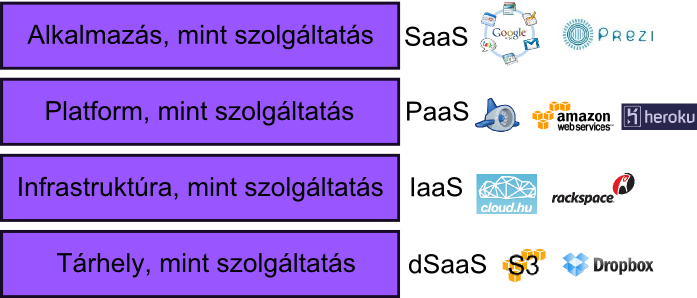
\includegraphics[width=0.5\textwidth]{figures/cloud_service_models.png}
\caption{A számítási felhő szolgáltatási modelljei \label{fig:cloud_service_models}}
\end{figure}
 
\subsubsection{Adattár, mint szolgáltatás (\foreignlanguage{english}{data-Storage-as-a-Service, dSaaS})}
Ezt a szolgáltatást nem minden irodalom szokta említeni, ám én itt mégis külön kezelném, hiszen ez a felhő legalapvetőbb szolgáltatása. Lényege, hogy online tárhelyet biztosít a felhasználóknak. Ilyen szolgáltatást nyújt pl. a \href{http://www.dropbox.com}{Dropbox.com} (főleg személyes felhasználásra, biztonsági mentés, megosztás céljából) vagy az \href{https://aws.amazon.com/s3/}{Amazon S3} (inkább nagy szolgáltatók használják).

A dSaaS oktatási rendszerek esetében sok, nagyméretű adatok esetén lehet előnyös, hiszen nem kell a saját szerverünkön tárolni ezeket, megspórolva ezzel saját adattároló rendszer kialakítását, üzemeltetését. Érdemes megjegyezni, hogy sok adatpéldány esetén is érdemes lehet hasonló szolgáltatás használata, hiszen ebben az esetben az autentikációhoz kötött adatoknál már nem kell a session-öket kezelni, az adatok elérhetőségét megadó URL már tartalmaz egy kódot, csökkentve ezzel a web és alkalmazás szerver terheltségét. 

\todo{dSaaS-ról még valami?}

\subsubsection{Infrastuktúra, mint szolgálatás (\foreignlanguage{english}{Infrastructure-as-a-Service, IaaS})}

Az infrastruktúra, mint szolgáltatás az előfizető számára rendelkezésre bocsájt olyan feldolgozási, tárhely, hálózati és egyéb alapvető számítási erőforrásokat, ahol az előfizető képes telepíteni és futtatni tetszőleges szoftvert, amely szoftver magába foglalhatja magát az operációs rendszert és egyéb alkalmazásokat is. Az előfizető nem kezeli a szolgáltatás alapjául szolgáló infrastruktúrát, de irányítása alá tartozik az operációs rendszer, a tárhely és a telepített alkalmazások; esetleg korlátozottan hálózati komponensek (pl. tűzfalak).\cite{nistsp800-145}

Az IaaS az infrastruktúra (számítási erőforrások és tárhely) bérbeadása. Ez nem csak virtualizált számítógépeket jelent garantált számítási teljesítménnyel, de fenntartott sávszélességet a tárhely és az internet elérésnek is. Lényegében a lehetősége egy számítógép vagy adatközpont bérvételének, specifikált szolgáltatásminőség (QoS) megkötésekkel, amelyekkel képesek vagyunk egy tetszőleges operációs rendszer és szoftver futtatására.\cite{ccwlinux}

A legismertebb IaaS szolgáltatók az Amazon (Amazon EC2: \href{https://aws.amazon.com/ec2/}{https://aws.amazon.com/ec2/}) és a Rackspace (\href{http://www.rackspace.com/}{http://www.rackspace.com/}) A különböző IaaS-t nyújtó cégek szolgáltatásai nagyjából hasonlóak. A felhasználók előre beállított konfigurációk közül választhatják ki a nekik megfelelőt. Ezek a konfigurációk erőforrásokban, előre telepített operációs rendszerekben\footnote{Nem csak ingyenes OS-eket, de fizetős (pl. Microsoft) termékeket is igénybe vehetünk, ahol a licenc ára a felhasználás idejének arányában oszlik el, így nekünk nem kell foglalkoznunk a szoftver beszerzésével.} és árban különbözhetnek.

Egy LMS üzemeltetésével foglalkozó szervezet esetén rengeteg előnyt jelenthet a rendszer felhőben való üzemeltetése. Az IaaS elasztikus tulajdonságának köszönhetően gyorsan tudjuk a változó erőforrásigényeket kielégíteni. Ezek a szolgáltatások idő és teljesítmény alapú számlázást használnak, így jó közelítéssel előre meghatározhatóak a költségek. A szolgáltatók nagy rendelkezésre állást biztosítanak, így nem fordulhat elő, hogy a rendszerünk nem érhető el. Természetesen ezen a szinten még szükségünk van IT munkatársakra, hiszen a rendszert fel kell építeni, és szoftveres szinten karban kell tartani, de már a hardveres szint hiánya is egyszerűsítheti a munkát.

\todo{IaaS-ról még valami?}

\subsubsection{Platform, mint szolgáltatás (\foreignlanguage{english}{Platform-as-a-Service, PaaS})}

A platform, mint szolgáltatás az előfizető számára rendelkezésre bocsájtja annak a lehetőségét, hogy olyan a felhasználó által létrehozott vagy beszerzett alkalmazásokat telepítsen a felhő infrastruktúrára, amelyek a szolgáltató által támogatott programozási nyelvet, könyvtárakat, szolgáltatásokat és eszközöket használnak. A felhasználó nem kezeli vagy vezérli a szolgáltatás alapjául szolgáló infrastruktúrát, beleértve a hálózatot, szervereket, operációs rendszereket, vagy a tárhelyet, de irányítással rendelkezik a telepített alkalmazások és esetleg a konfigurációs beállítások felett. Ezen felül nincs kizárva  annak a lehetősége, hogy az előfizető más forrásból származó kompatibilis programozási nyelveket, könyvtárakat, szolgáltatásokat és eszközöket használjon.\cite{nistsp800-145}

A PaaS hasonló az IaaS-hoz, de olyan operációs rendszereket és kötelező szolgáltatásokat foglal magába, amelyek egy sajátos alkalmazásra fókuszálnak. Például PaaS-ként tekinthetünk egy virtualizált szerver, tárhelyszolgáltatás, operációs rendszer és alkalmazás halmazt (ami tipikusan egy virtuális gép fájl formátumban, pl. a VMware .vmdk állománya), hozzáféréssel a szükséges szolgáltatásokhoz, mint amilyen például egy MySQL adatbázis vagy egyéb, specializált helyi erőforrás. Más szavakkal a PaaS egy IaaS, testre szabott szoftver stackkel egy adott alkalmazáshoz.\cite{ccwlinux}

A piacon több PaaS szolgáltató találunk, ezek közül szedtem össze néhányat \aref{tab:paas_providers}.~táblázatba.

\begin{table}[h]
	\caption{Néhány ismertebb PaaS szolgáltató}
	\centering
	\small
	\begin{tabular}{| p{4cm} | p{5.5cm} | p{4cm} |}
		\hline
		\rowcolor{MyTableColor} \textbf{Szolgáltató} & \textbf{URL} & \textbf{Platform} \\
		\hline
		Google AppEngine & \href{https://appengine.google.com}{https://appengine.google.com} & Python, Java, Go \\ 
		\hline
		Heroku & \href{http://www.heroku.com/}{http://www.heroku.com/} & Ruby, Node.js, Clojure, Java, Python, Scala \\
		\hline
		Epio & \href{https://www.ep.io/}{https://www.ep.io/} & Python (Django, Pylons, Pyramid, Flask, Trac) \\
		\hline
		Zend PHP Cloud Application Platform & \href{http://www.zend.com/en/products/php-cloud/}{http://www.zend.com/en/products/php-cloud/} & PHP\\
		\hline
		SpringSource & \href{http://www.springsource.com/}{http://www.springsource.com/} & Java (Groovy, Grails)\\
		\hline
	\end{tabular}
	\normalsize
	\label{tab:paas_providers}
\end{table}
 

A Zend PHP Cloud Application Platform nem igazi szolgáltatás, csak egy platform, amelyet pl. Amazon EC2-re lehet telepíteni, mint ahogy a SpringSource is szintén egy telepíthető platform VMware vFabric Cloud Application Platform alapokon.

A PaaS egy környezetet biztosít az alkalmazásunknak, amely lehet akár egy LMS is. Az IaaS-szel ellentétben itt már nem kell foglalkoznunk az OS üzemeltetésével járó feladatokkal, csak is magával az LMS alkalmazással, amelyet nekünk kell telepíteni, vagy adott esetben a platformra lefejleszteni. Ugyanakkor az IaaS-nél megjelent előnyök itt is érvényesek, mind üzemeltetés, mind költség szempontjából.

\todo{PaaS-ról még valami?}

\subsubsection{Szoftver, mint szolgáltatás (\foreignlanguage{english}{Software-as-a-Service,SaaS})}

\foreignlanguage{english}{''The capability provided to the consumer is to use the provider’s applications running on a cloud infrastructure. A cloud infrastructure is the collection of hardware and software that enables the five essential characteristics of cloud computing. The cloud infrastructure can be viewed as containing both a physical layer and an abstraction layer. The physical layer consists of the hardware resources that are necessary to support the cloud services being provided, and typically includes server, storage and network components. The abstraction layer consists of the software deployed across the physical layer, which manifests the essential cloud characteristics.  Conceptually the abstraction layer sits above the physical layer. The applications are accessible from various client devices through either a thin client interface, such as a web browser (e.g., web-based email), or a program interface. The consumer does not manage or control the underlying cloud infrastructure including network, servers, operating systems, storage, or even individual application capabilities, with the possible exception of limited user-specific application configuration settings.''}\cite{nistsp800-145}

\todo{SaaS}

\todo{Deployment Models}
